% Options for packages loaded elsewhere
\PassOptionsToPackage{unicode}{hyperref}
\PassOptionsToPackage{hyphens}{url}
%
\documentclass[
]{article}
\usepackage{amsmath,amssymb}
\usepackage{iftex}
\ifPDFTeX
  \usepackage[T1]{fontenc}
  \usepackage[utf8]{inputenc}
  \usepackage{textcomp} % provide euro and other symbols
\else % if luatex or xetex
  \usepackage{unicode-math} % this also loads fontspec
  \defaultfontfeatures{Scale=MatchLowercase}
  \defaultfontfeatures[\rmfamily]{Ligatures=TeX,Scale=1}
\fi
\usepackage{lmodern}
\ifPDFTeX\else
  % xetex/luatex font selection
\fi
% Use upquote if available, for straight quotes in verbatim environments
\IfFileExists{upquote.sty}{\usepackage{upquote}}{}
\IfFileExists{microtype.sty}{% use microtype if available
  \usepackage[]{microtype}
  \UseMicrotypeSet[protrusion]{basicmath} % disable protrusion for tt fonts
}{}
\makeatletter
\@ifundefined{KOMAClassName}{% if non-KOMA class
  \IfFileExists{parskip.sty}{%
    \usepackage{parskip}
  }{% else
    \setlength{\parindent}{0pt}
    \setlength{\parskip}{6pt plus 2pt minus 1pt}}
}{% if KOMA class
  \KOMAoptions{parskip=half}}
\makeatother
\usepackage{xcolor}
\usepackage[margin=1in]{geometry}
\usepackage{graphicx}
\makeatletter
\def\maxwidth{\ifdim\Gin@nat@width>\linewidth\linewidth\else\Gin@nat@width\fi}
\def\maxheight{\ifdim\Gin@nat@height>\textheight\textheight\else\Gin@nat@height\fi}
\makeatother
% Scale images if necessary, so that they will not overflow the page
% margins by default, and it is still possible to overwrite the defaults
% using explicit options in \includegraphics[width, height, ...]{}
\setkeys{Gin}{width=\maxwidth,height=\maxheight,keepaspectratio}
% Set default figure placement to htbp
\makeatletter
\def\fps@figure{htbp}
\makeatother
\setlength{\emergencystretch}{3em} % prevent overfull lines
\providecommand{\tightlist}{%
  \setlength{\itemsep}{0pt}\setlength{\parskip}{0pt}}
\setcounter{secnumdepth}{-\maxdimen} % remove section numbering
\ifLuaTeX
  \usepackage{selnolig}  % disable illegal ligatures
\fi
\IfFileExists{bookmark.sty}{\usepackage{bookmark}}{\usepackage{hyperref}}
\IfFileExists{xurl.sty}{\usepackage{xurl}}{} % add URL line breaks if available
\urlstyle{same}
\hypersetup{
  pdftitle={DRAFT: Final Project},
  pdfauthor={Katie Perez},
  hidelinks,
  pdfcreator={LaTeX via pandoc}}

\title{DRAFT: Final Project}
\author{Katie Perez}
\date{2024-02-29}

\begin{document}
\maketitle

Line graph I aim to illustrate the fluctuations in enrollment over time
through this visualization. To elucidate the trends, I propose focusing
on selected colleges and universities. From the plot, it's evident that
both UO and OSU have experienced enrollment growth, whereas other
institutions depict a marginal decline. I've assigned distinct colors to
each line based on the official brand hex codes of the respective
institutions. While adding annotations with school names could enhance
clarity, I am concerned it might overly clutter the visualization.

\begin{verbatim}
## File .here already exists in /Users/kperez/Documents/Winter 2024/EDLD 652/Final project
\end{verbatim}

\begin{verbatim}
## Warning: The `<scale>` argument of `guides()` cannot be `FALSE`. Use "none" instead as
## of ggplot2 3.3.4.
## This warning is displayed once every 8 hours.
## Call `lifecycle::last_lifecycle_warnings()` to see where this warning was
## generated.
\end{verbatim}

Paired bar chart applicants and enrolled

This paired bar graph illustrates both applicants and enrollees,
highlighting the shift in numbers between the two categories. The
transition from applicants to enrollees presents an intriguing insight.
Furthermore, the total number of applicants each institution receives
holds its own significance. To further enrich the analysis, it would be
beneficial to incorporate the number of acceptances into the
visualization. Applicant and enrollment data was not available for the
2-year institutions, so I omitted them from this visualization.

\begin{verbatim}
##   unitid                 institution.name year HD2022.State.abbreviation
## 1 208275  Blue Mountain Community College 2022                    Oregon
## 2 208318 Central Oregon Community College 2022                    Oregon
## 3 208390      Chemeketa Community College 2022                    Oregon
## 4 208406      Clackamas Community College 2022                    Oregon
## 5 208415        Clatsop Community College 2022                    Oregon
## 6 208646        Eastern Oregon University 2022                    Oregon
##   HD2022.Sector.of.institution ADM2022.Applicants.total ADM2022.Enrolled.total
## 1               Public, 2-year                       NA                     NA
## 2               Public, 2-year                       NA                     NA
## 3               Public, 2-year                       NA                     NA
## 4               Public, 2-year                       NA                     NA
## 5               Public, 2-year                       NA                     NA
## 6      Public, 4-year or above                     1015                    252
##   EF2022D.Full.time.fall.2021.cohort
## 1                                238
## 2                                493
## 3                               1161
## 4                                509
## 5                                 89
## 6                                244
##   EF2022D.Students.from.the.full.time.adjusted.fall.2021.cohort.enrolled.in.fall.2022
## 1                                                                                 145
## 2                                                                                 281
## 3                                                                                 726
## 4                                                                                 279
## 5                                                                                  51
## 6                                                                                 165
##   EF2022D.Full.time.retention.rate..2022
## 1                                     61
## 2                                     57
## 3                                     63
## 4                                     55
## 5                                     57
## 6                                     68
\end{verbatim}

\begin{verbatim}
##                           institution.name year ADM2022.Applicants.total
## 6                Eastern Oregon University 2022                     1015
## 26 Oregon State University-Cascades Campus 2022                     2097
## 17              Southern Oregon University 2022                     2126
## 21               Western Oregon University 2022                     3262
## 11          Oregon Institute of Technology 2022                     4570
## 15               Portland State University 2022                     7926
##    ADM2022.Enrolled.total
## 6                     252
## 26                    188
## 17                    567
## 21                    563
## 11                    463
## 15                   1634
\end{verbatim}

\begin{verbatim}
## Warning in mean.default(X[[i]], ...): argument is not numeric or logical:
## returning NA

## Warning in mean.default(X[[i]], ...): argument is not numeric or logical:
## returning NA

## Warning in mean.default(X[[i]], ...): argument is not numeric or logical:
## returning NA

## Warning in mean.default(X[[i]], ...): argument is not numeric or logical:
## returning NA

## Warning in mean.default(X[[i]], ...): argument is not numeric or logical:
## returning NA

## Warning in mean.default(X[[i]], ...): argument is not numeric or logical:
## returning NA

## Warning in mean.default(X[[i]], ...): argument is not numeric or logical:
## returning NA

## Warning in mean.default(X[[i]], ...): argument is not numeric or logical:
## returning NA

## Warning in mean.default(X[[i]], ...): argument is not numeric or logical:
## returning NA

## Warning in mean.default(X[[i]], ...): argument is not numeric or logical:
## returning NA

## Warning in mean.default(X[[i]], ...): argument is not numeric or logical:
## returning NA

## Warning in mean.default(X[[i]], ...): argument is not numeric or logical:
## returning NA

## Warning in mean.default(X[[i]], ...): argument is not numeric or logical:
## returning NA

## Warning in mean.default(X[[i]], ...): argument is not numeric or logical:
## returning NA

## Warning in mean.default(X[[i]], ...): argument is not numeric or logical:
## returning NA

## Warning in mean.default(X[[i]], ...): argument is not numeric or logical:
## returning NA
\end{verbatim}

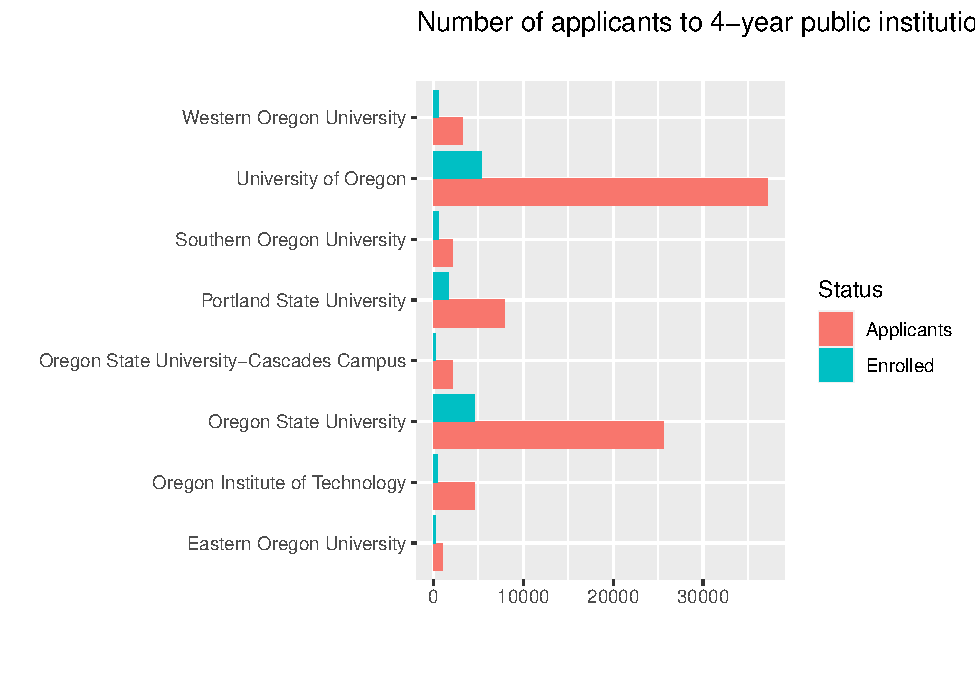
\includegraphics{Final_files/figure-latex/unnamed-chunk-1-1.pdf}

Bar Plot

In this plot, I analyze the retention rates of Oregon's public
universities. Although I categorized the institutions into 2-year and
4-year groups in the dataset, this grouping did not translate into the
plot. I will continue refining my code to accurately represent these
distinctions.To enhance the informative value of this visualization, I
propose expanding the timeframe to encompass multiple years. Facet
wrapping across several years could offer a comprehensive view.
Additionally, it's crucial to note that the retention rates presented
are proportions. I anticipate that examining retention rates alongside
data on applicants and enrollees will provide valuable insights into
enrollment dynamics.

\begin{verbatim}
##   unitid                 institution.name year HD2022.State.abbreviation
## 1 208275  Blue Mountain Community College 2022                    Oregon
## 2 208318 Central Oregon Community College 2022                    Oregon
## 3 208390      Chemeketa Community College 2022                    Oregon
## 4 208406      Clackamas Community College 2022                    Oregon
## 5 208415        Clatsop Community College 2022                    Oregon
## 6 208646        Eastern Oregon University 2022                    Oregon
##   HD2022.Sector.of.institution ADM2022.Applicants.total ADM2022.Enrolled.total
## 1               Public, 2-year                       NA                     NA
## 2               Public, 2-year                       NA                     NA
## 3               Public, 2-year                       NA                     NA
## 4               Public, 2-year                       NA                     NA
## 5               Public, 2-year                       NA                     NA
## 6      Public, 4-year or above                     1015                    252
##   EF2022D.Full.time.fall.2021.cohort
## 1                                238
## 2                                493
## 3                               1161
## 4                                509
## 5                                 89
## 6                                244
##   EF2022D.Students.from.the.full.time.adjusted.fall.2021.cohort.enrolled.in.fall.2022
## 1                                                                                 145
## 2                                                                                 281
## 3                                                                                 726
## 4                                                                                 279
## 5                                                                                  51
## 6                                                                                 165
##   EF2022D.Full.time.retention.rate..2022
## 1                                     61
## 2                                     57
## 3                                     63
## 4                                     55
## 5                                     57
## 6                                     68
\end{verbatim}

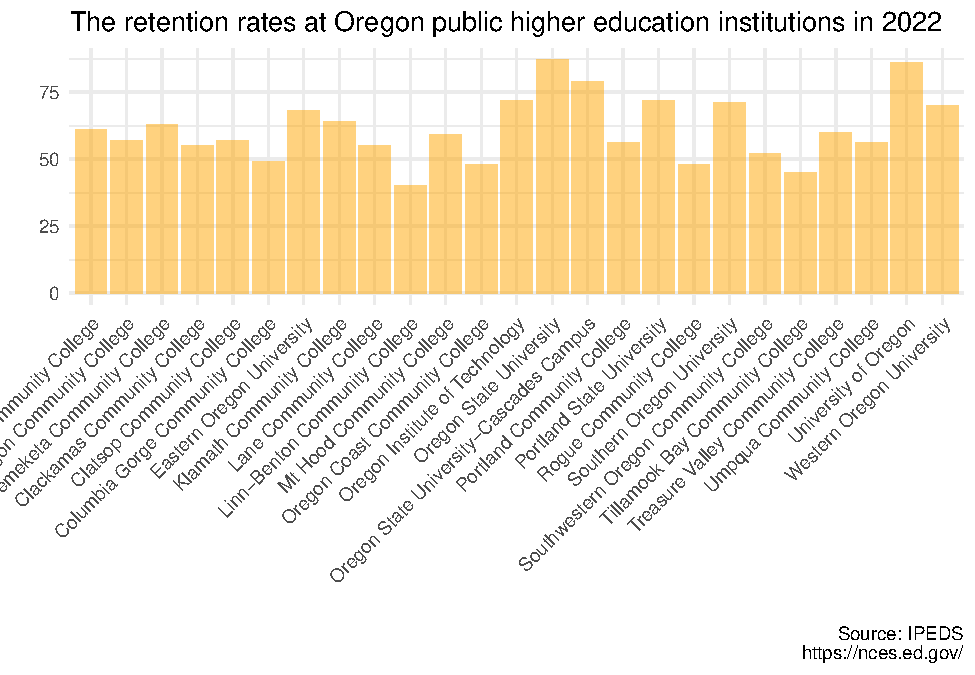
\includegraphics{Final_files/figure-latex/unnamed-chunk-2-1.pdf}

\end{document}
